%!TEX root=../document.tex

\section{Aufgabestellung}
Dieses Protokoll-Template soll helfen den Laborübungsteil entsprechend dokumentieren zu können.
Diese Vorlage ist in \LaTeX{}  verfasst.

\subsection{Ziele}
Hier werden die zu erwerbenden Kompetenzen und deren Deskriptoren beschrieben.
Diese werden von den unterweisenden Lehrkräften vorgestellt.

Dies kann natürlich auch durch eine Aufzählung erfolgen:

\begin{itemize}
	\item \textbf{Lorem ipsum:} dolor sit amet, consetetur sadipscing elitr
	\item \textbf{Sed diam:} nonumy eirmod tempor invidunt ut labore et dolore magna aliquyam erat
	\item \textbf{Ut labore:} et dolore magna aliquyam erat, sed diam voluptua
\end{itemize}


\subsection{Voraussetzungen}
\lipsum[4]

\begin{figure}[!h]
	\begin{center}
		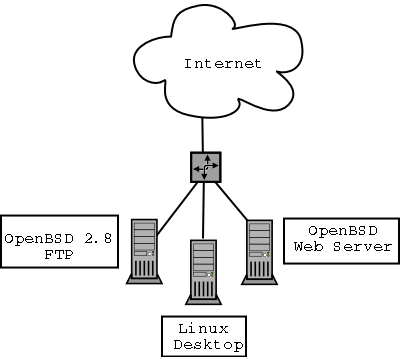
\includegraphics[width=0.4\linewidth]{images/home_network.png}
		\caption{Figure \cite{example}}
		\label{broker}
	\end{center}
\end{figure}
